% Chapter 4
\chapter{SYSTEM DESIGN} % All Chapter headings in ALL CAPS


\section{Components in the project}
\subsection{Hardware Components}
\begin{verbatim}
1. Raspberry pi microcomputer
2. L298n motor driver
3. Robot chassis
4. Wheels 
5. 12V battery
6. Male-female connecting wires
7. Wi-Fi modem/ router
8. Portable charger
9. 3G dongle
10. Microsoft Kinect 
11. Raspberry Pi camera module
\end{verbatim}
\subsection{Software Components}
\begin{verbatim}
1. Raspbian OS (Linux flavor for RPI)
2. Microsoft Kinect SDK 
3. Microsoft visual studio VNC server
4. SSH (Putty)
5. XRDP (remote desktop) VNC viewer 
6. Terminal emulator for android 
\end{verbatim}
\subsection{Programs}
\begin{verbatim}
a) Python program to move robot in the following directions:
1. Left
2. Right
3. Forward
4. Backward
5. Circular manner
b) Gesture detection and processing for the Kinect:
1. Swipe left
2. Swipe right
3. Mouse control 
4. Swipe up
5. Swipe down
6. Circle
c) C# SSH Connection 
\end{verbatim}

\section{Technology used}
\subsection{Raspberry-pi}
The robot is aimed to be controlled using the Raspberry-pi. Raspberry pi (RPI) is a credit card sized microcomputer that runs on a Linux based operating system loaded on its SD card . It is powered by the Broadcom BCM2835 system-on-a-chip (SoC) that includes a 32-bit ARM1176JZFS processor, clocked at 700MHz, and a Videocore IV GPU. It has 512 MB ram and can be over-clocked to 1000 MHz. It can connect to a network by using an external user-supplied USB Ethernet or Wi- Fi adapter. Furthermore, the raspberry-pi has two USB ports, an HDMI port, Audio In and out, RCA video output and GPIO Pins inbuilt. This contains an ARM1176JZFS (ARM11 using an ARMv6-architecture core) with floating point, running at 700Mhz. Apart from this, the Raspberry-pi can have a 5MP camera module mounted on it. Being Linux based, it gives the programmer more freedom to tweak with the various flavors of the Raspbian operating system.

\begin{figure}[H]
  \centering
  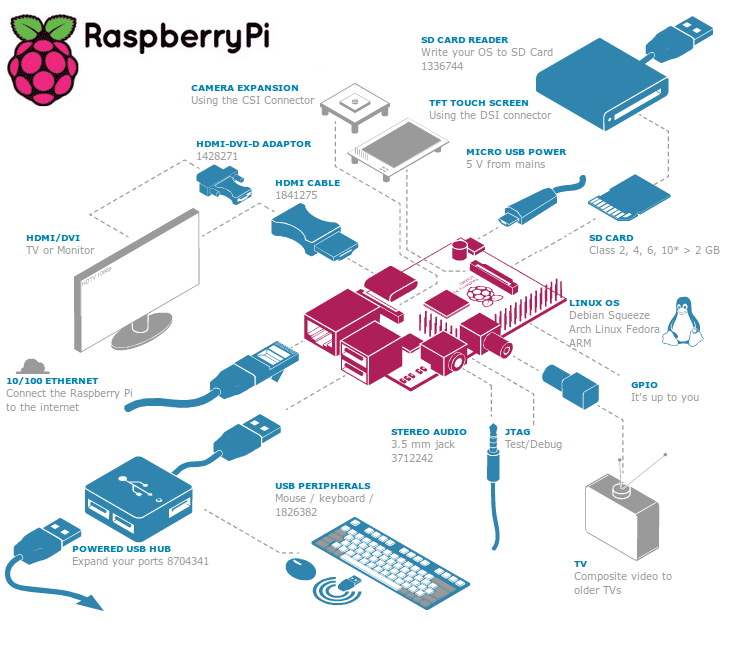
\includegraphics[width = 15cm, height = 12cm]{rpi.png}
  \caption{Raspberry Pi}
  \label{RPi}	
\end{figure}

\subsection{L298N Motor Driver}
The L298 is an integrated monolithic circuit in a 15-lead Multiwatt and PowerSO20 packages. It is a high voltage, high current dual full-bridge driver designed to accept standard TTL logic levels and drive inductive loads such as relays, solenoids, DC and stepping motors. Two enable inputs are provided to enable or disable the device independently of the input signals. The emitters of the lower transistors of each bridge are connected together and the corresponding external terminal can be used for the connection of an external sensing resistor. An additional supply input is provided so that the logic works at a lower voltage.

\begin{figure}[H]
  \centering
  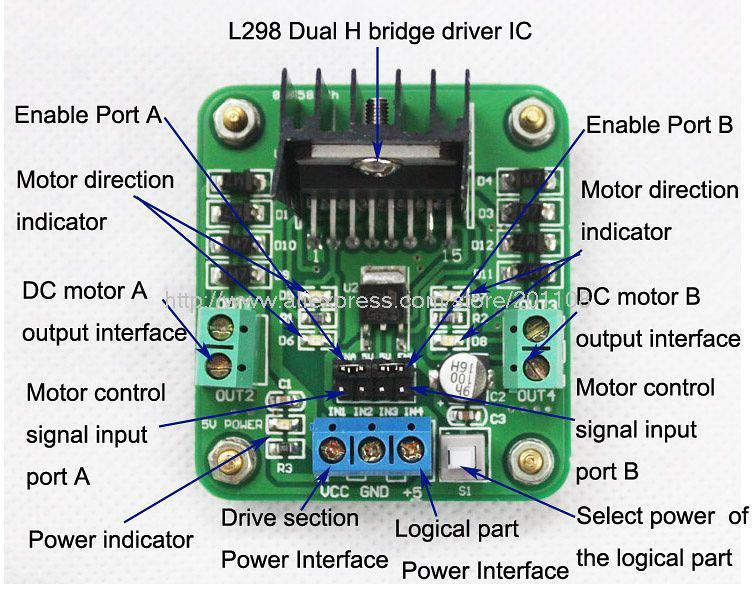
\includegraphics[width = 15cm, height = 12cm]{motor.jpg}
  \caption{L298N Motor Driver}
  \label{L298N motor driver}	
\end{figure}



\subsection{Microsoft Kinect}
Gesture and voice recognition is achieved using the Microsoft Kinect for Windows which is a motion sensing input device. The Kinect contains an RGB camera that stores three channel data in a 1280x960 resolution. This makes capturing a color image possible. It has an infrared (IR) emitter and an IR depth sensor. The emitter emits infrared light beams and the depth sensor reads the IR beams reflected back to the sensor. The reflected beams are converted into depth information measuring the distance between an object and the sensor. This makes capturing a depth image possible. The Kinect also has a multi-array microphone, which contains four microphones for capturing sound. Because there are four microphones, it is possible to record audio as well as find the location of the sound source and the direction of the audio wave. Finally, there is a 3-axis accelerometer configured for a 2G range, where G is the acceleration due to gravity. It is possible to use the accelerometer to determine the current orientation of the Kinect.

\begin{figure}[H]
  \centering
  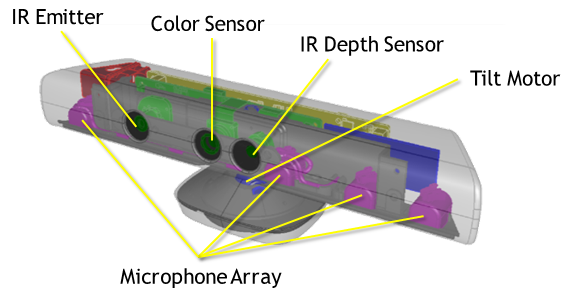
\includegraphics[width = 13cm, height = 7cm]{kinect.png}
  \caption{Schematic Diagram of Microsoft Kinect}
  \label{kinect}	
\end{figure}

\subsection{RPI Camera}
The Raspberry Pi camera board contains a 5 Mega Pixel sensor, and connects via a ribbon cable to the CSI connector on the Raspberry Pi. The video and still image quality is better than a USB webcam of similar price. The "Pi NoIR" version of the camera was released is what we are using for the project. It has the same sensor with the IR filter removed, and a black PCB. With no IR filter, it can see near-IR wavelengths (700 - 1000 nm) like a security camera, with the tradeoff of poor colour rendition. It is otherwise the same and uses the same software as the normal Pi camera.

\begin{figure}[H]
  \centering
  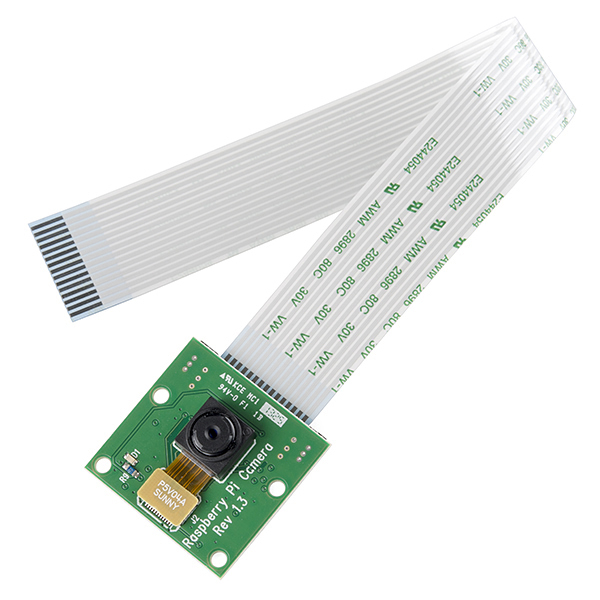
\includegraphics[width = 7cm, height = 6cm]{camera.jpg}
  \caption{Raspberry-pi camera}
  \label{RPI camera}	
\end{figure}

\section{Block Diagram}

\begin{figure}[H]
  \centering
  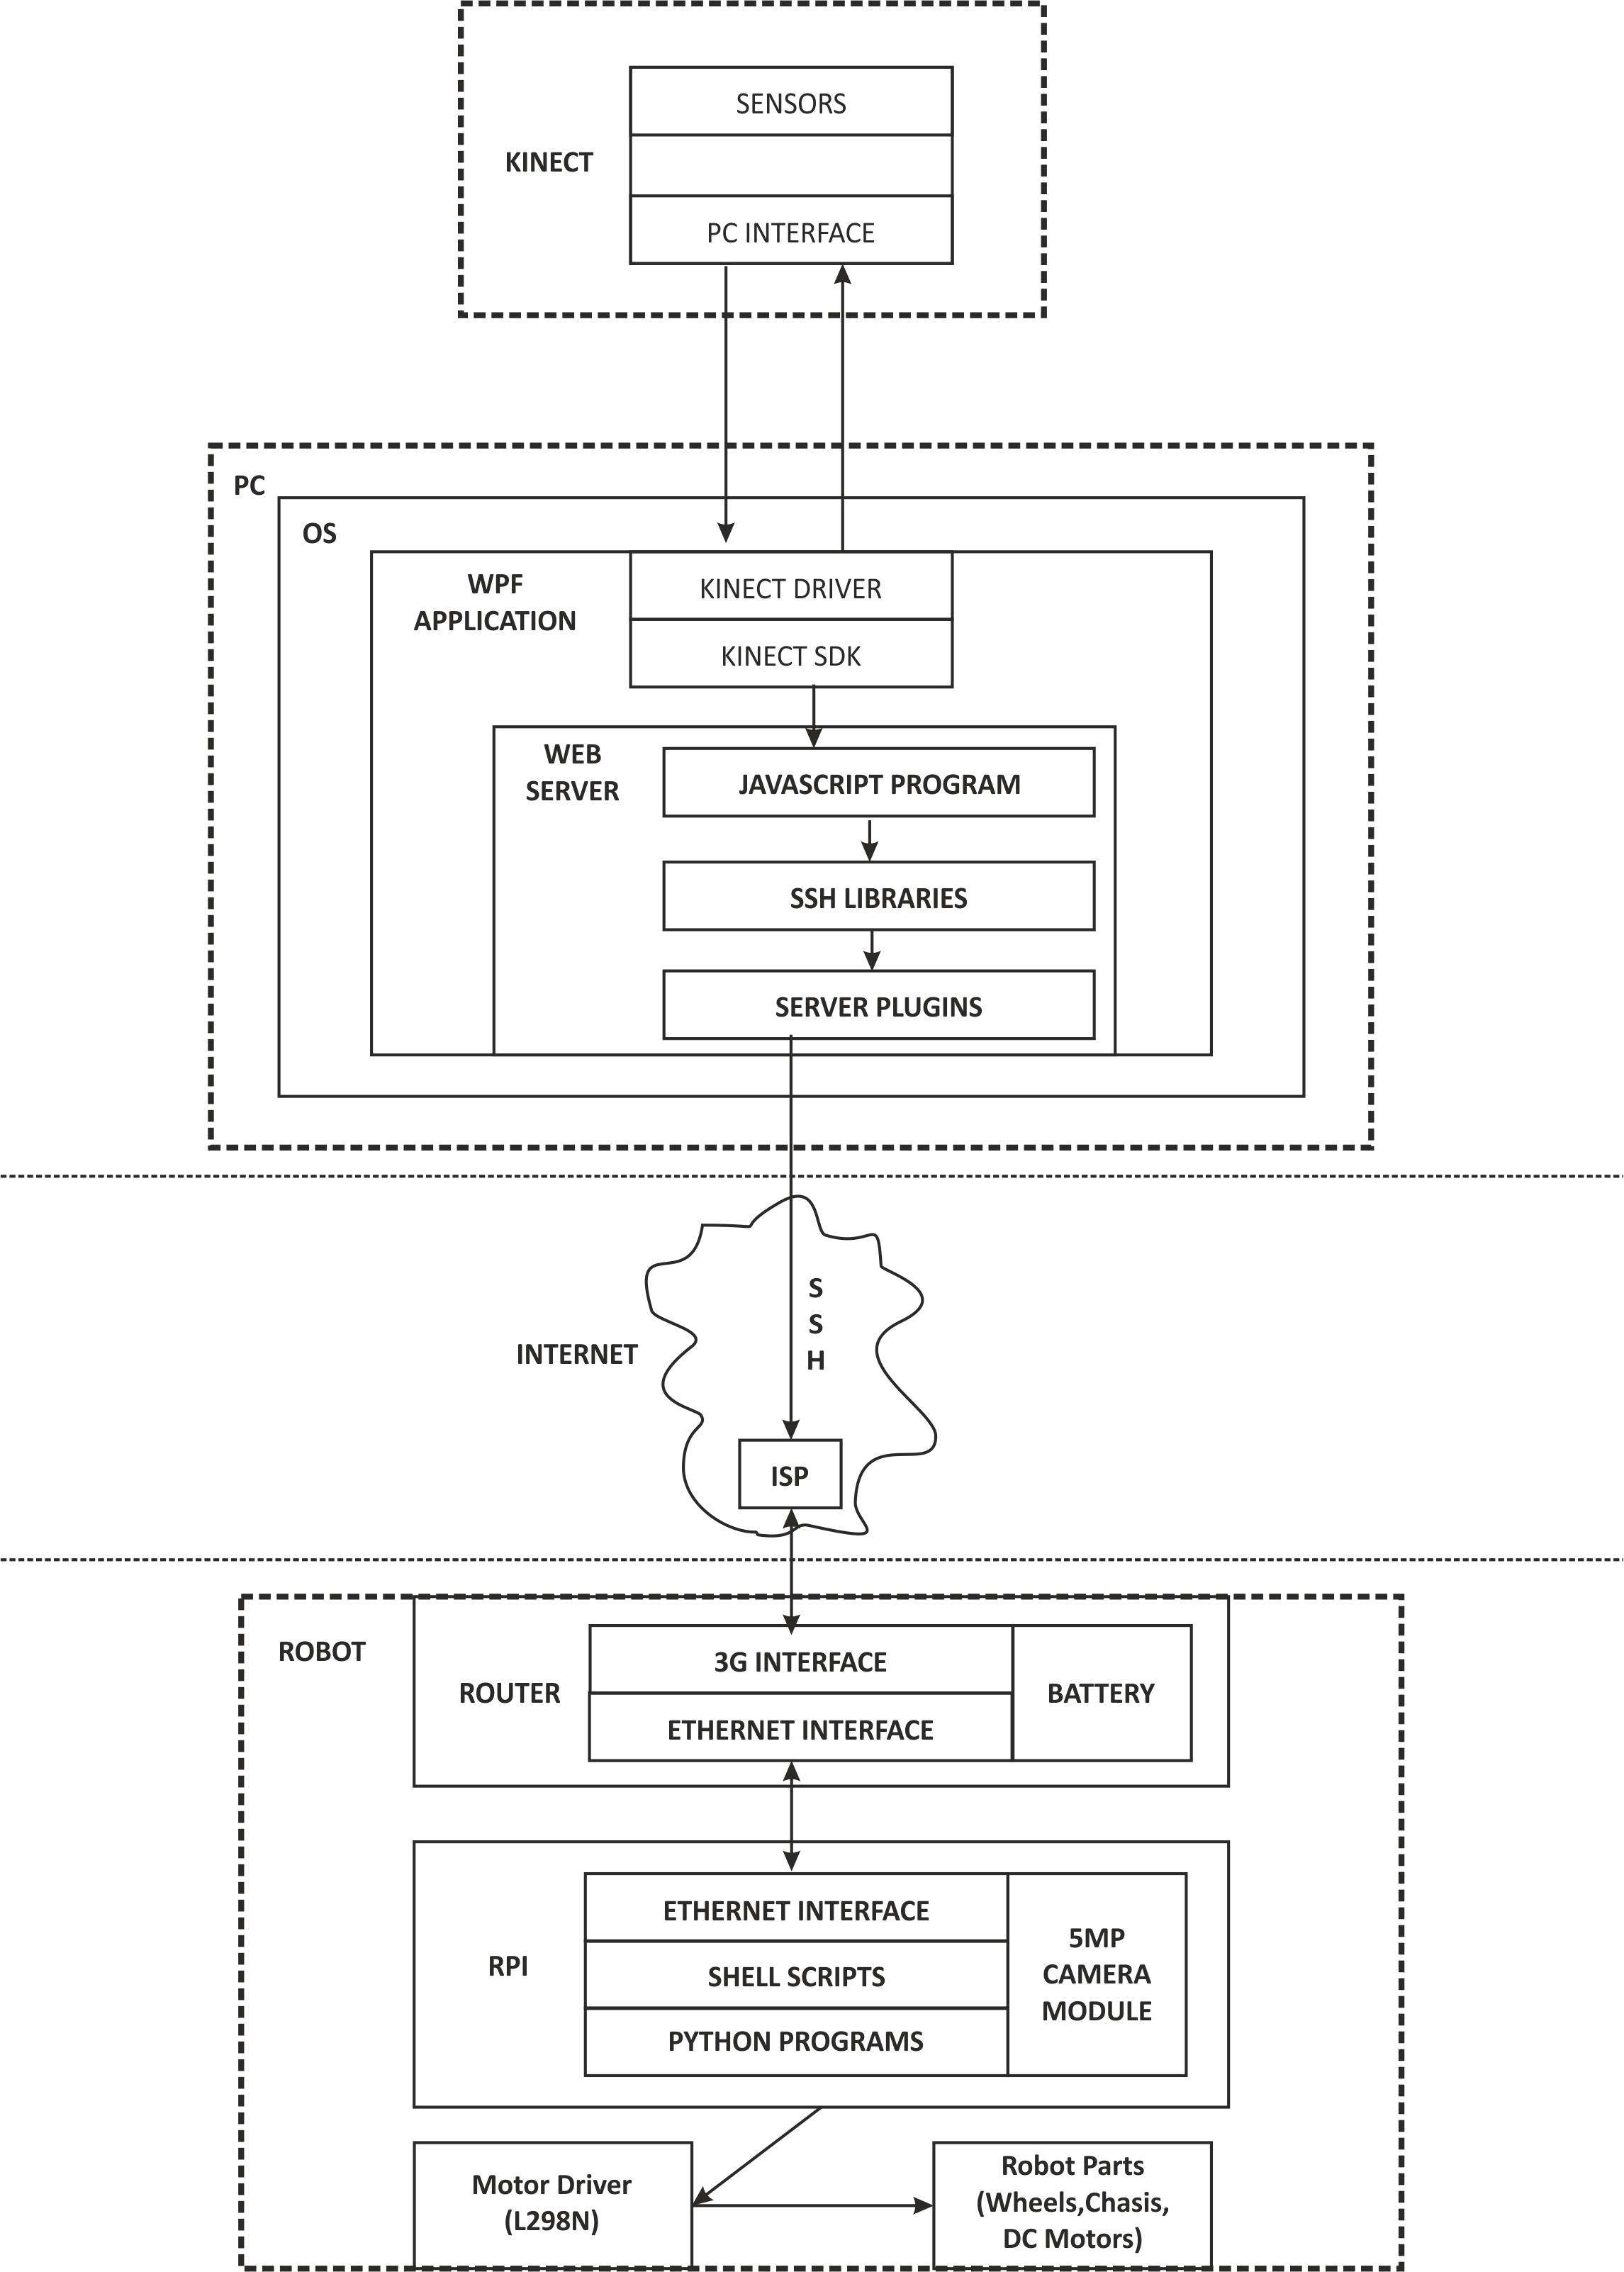
\includegraphics[width = 15cm, height = 16cm]{Blocks.jpg}
  \caption{Block Digram}
  \label{block}	
\end{figure}


\section{Flow Diagram}



\begin{figure}[H]
  \centering
  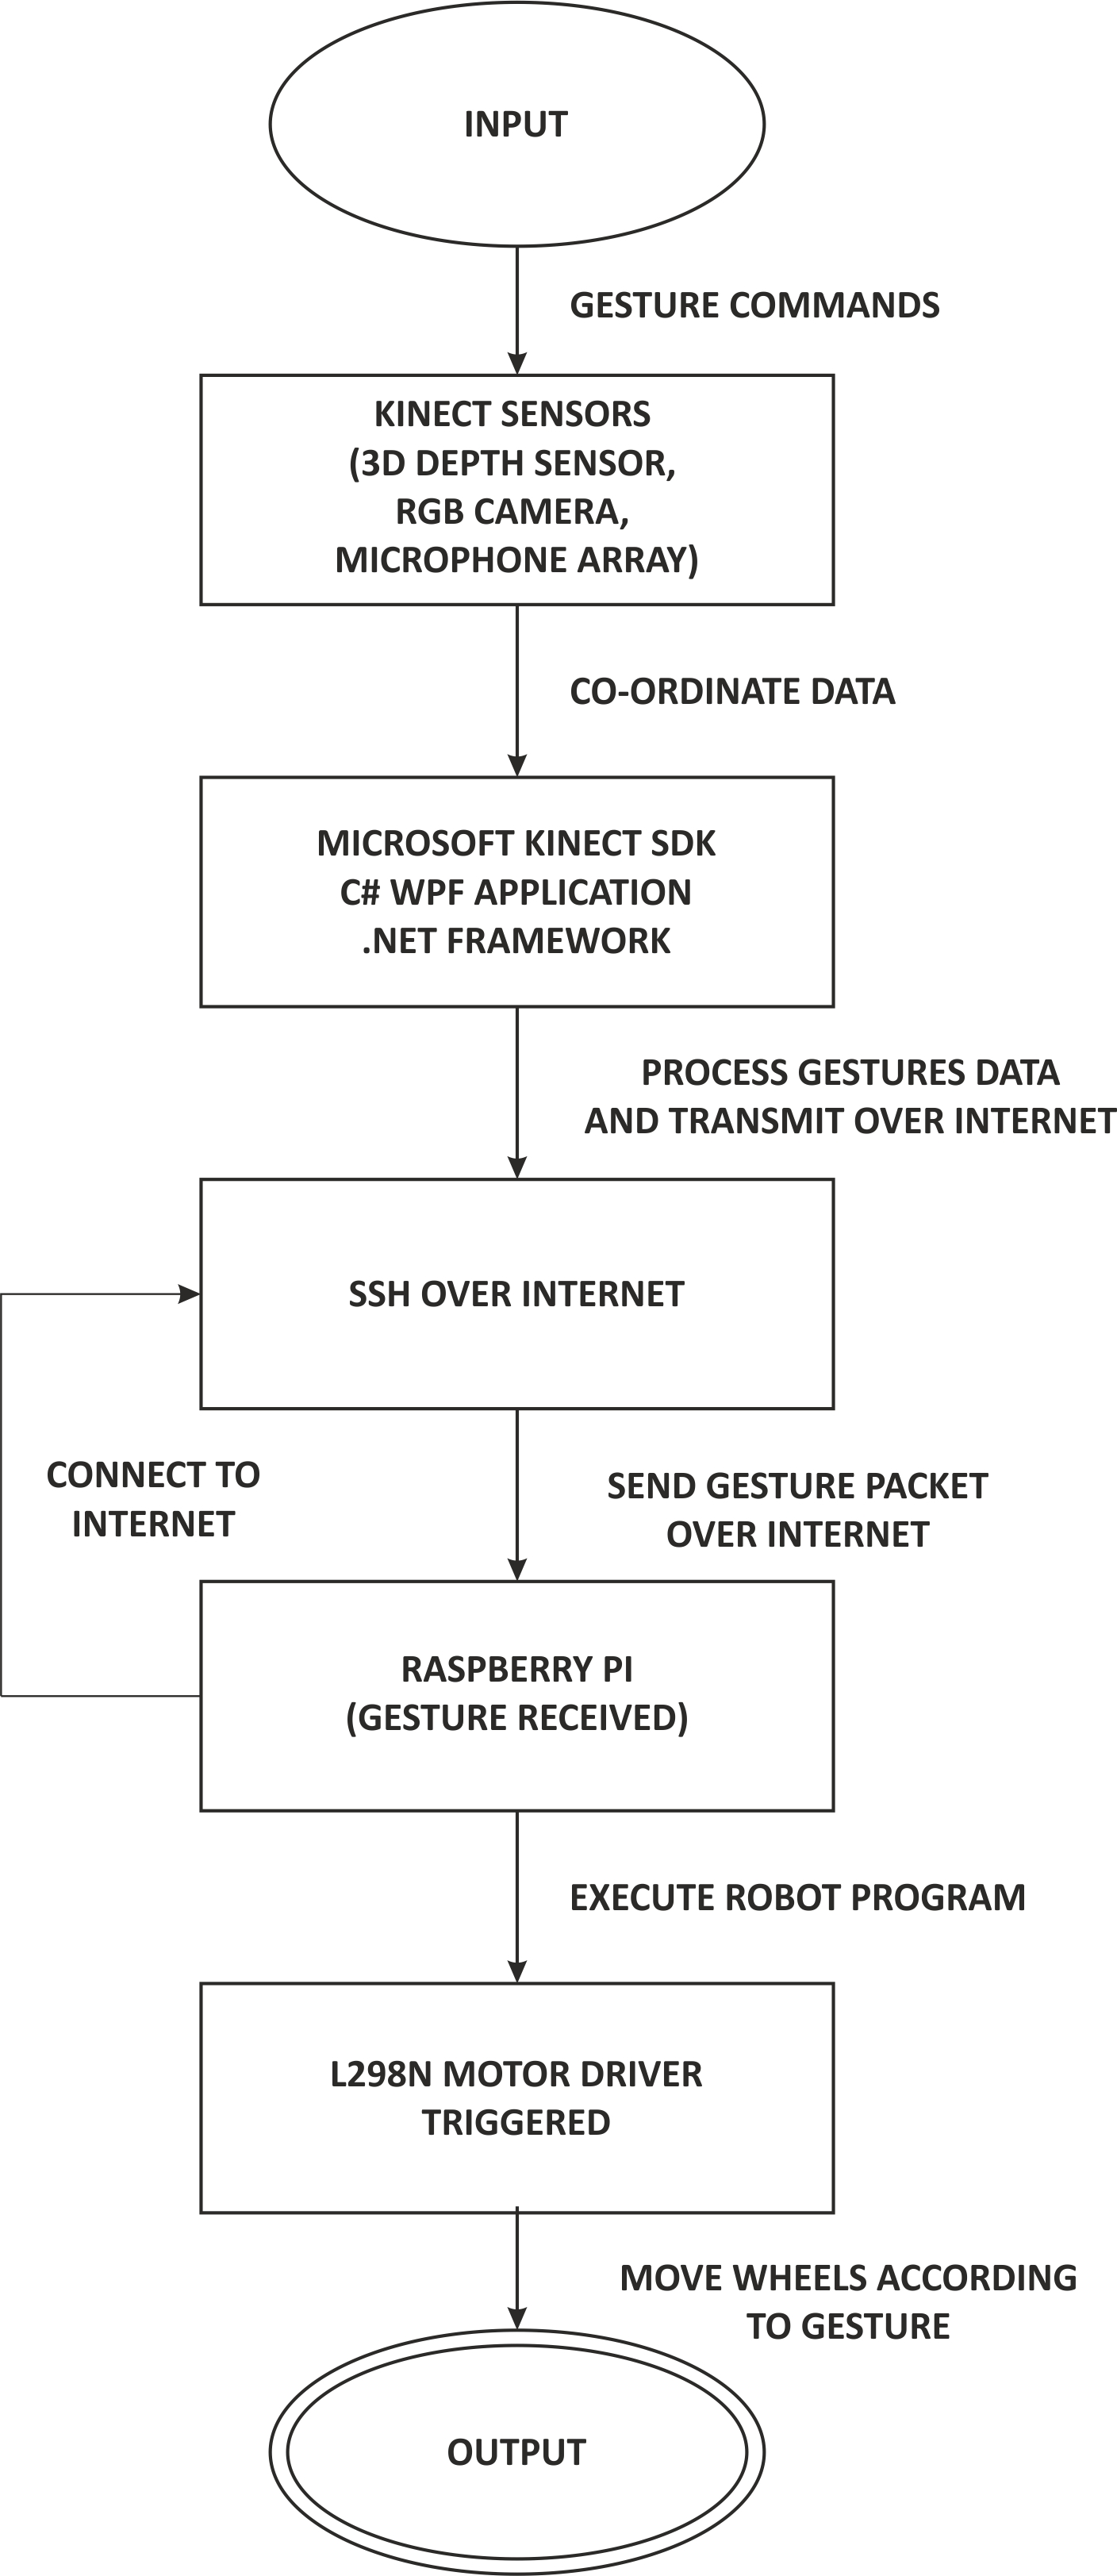
\includegraphics[width = 8cm, height = 19cm]{Flows.jpg}
  \caption{Flow Diagram from Input to Output}
  \label{Flow}	
\end{figure}
\textbf{Description of Flow Diagram}
\newline
The user provides a gesture or a voice command as input. This is captured by the various sensors present on the Microsoft Kinect. The coordinates of the gestures are then processed by the SDK on the PC, to recognize the nature of the gesture i.e Swipe Left, Swipe Right etc. The confirmed gesture is then passed on to the WPF application which processes it and sends as gesture packets over the internet. These gesture packets are received by the Internet Web Server and sent to the Raspberry-pi client. At all times, the Raspberry -pi is connected to the internet to communicate with the web-server. Upon receiving the gesture, the Raspberry-pi executes the Robot program written in Python. This triggers the L2N8N motor driver which is responsible for controlling the wheels of the robot. Depending on the gesture, the robot moves in the desired direction. Thus the final output is the motion of the robot as directed by the user.





